\documentclass[10pt]{beamer}
\setbeamertemplate{caption}[numbered]
\usepackage[utf8]{inputenc}
\usepackage{graphicx}
\usepackage{hyperref}
\usepackage {mathtools}
\usetheme{CambridgeUS}
\usecolortheme{dolphin}
\usepackage{circuitikz}
\usepackage{xcolor}

\renewcommand{\vec}[1]{\boldsymbol{\mathbf{#1}}}
\newcommand{\myvec}[1]{\ensuremath{\begin{pmatrix}#1\end{pmatrix}}}
\providecommand{\norm}[1]{\left\lVert#1\right\rVert}
\providecommand{\brak}[1]{\ensuremath{\left(#1\right)}}



\definecolor{myNewColorA}{RGB}{242,85,37}
\definecolor{myNewColorB}{RGB}{247,124,40}
\definecolor{myNewColorC}{RGB}{255,209,84}
\setbeamercolor*{palette primary}{bg=myNewColorC}
\setbeamercolor*{palette secondary}{bg=myNewColorB, fg = white}
\setbeamercolor*{palette tertiary}{bg=myNewColorA, fg = white}
\setbeamercolor*{titlelike}{fg=myNewColorA}
\setbeamercolor*{title}{bg=myNewColorA, fg = white}
\setbeamercolor*{item}{fg=myNewColorA}
\setbeamercolor*{caption name}{fg=myNewColorA}
\setbeamercolor*{block title}{use=structure,fg=white,bg=myNewColorB}
\setbeamercolor*{block body}{use=structure,fg=black,bg=myNewColorC}
\usefonttheme{professionalfonts}

%------------------------------------------------------------

\setbeamerfont{title}{size=\large}
\setbeamerfont{subtitle}{size=\small}
\setbeamerfont{author}{size=\small}
\setbeamerfont{date}{size=\small}
\setbeamerfont{group}{size = \small}
\setbeamerfont{institute}{size=\small}
\title{PT-100 Project}
\subtitle{EE2802 | Machine Learning}

\author[Jaswanth]{Jaswanth Chowdary Madala (EE20BTECH11025)}

\institute{IIT Hyderabad}
\date{\today}

\AtBeginSection[]{
  \begin{frame}
  \vfill
  \centering
  \begin{beamercolorbox}[sep=8pt,center,shadow=true,rounded=true]{title}
    \usebeamerfont{title}\insertsectionhead\par%
  \end{beamercolorbox}
  \vfill
  \end{frame}
}

%------------------------------------------------------------

\begin{document}
\maketitle

\begin{frame}{Contents}
    \tableofcontents
\end{frame}

%------------------------------------------------------------

\section{Introduction}
\begin{frame}{Introduction}
	\setbeamercovered{transparent}
    \begin{itemize}
    \item  The project is about using machine learning techniques to model the voltage-temperature characteristics of the PT-100 \vspace{0.25cm}
    \item In this project, we will apply Linear Regression using the least squares method to model the voltage-temperature characteristics of the PT-100 sensor 
    \end{itemize} 
\end{frame}

%------------------------------------------------------------

\section{PT-100 Sensor}
\begin{frame}{PT-100 Sensor}
	\setbeamercovered{transparent}
	\begin{itemize}
	\item The PT-100 sensor is a commonly used temperature sensor that is based on the resistance-temperature relationship of platinum \vspace{0.25cm}
	\item The characteristic equation of voltage vs Temperature is given by the Callendar-Van Dusen equation
\begin{align}
    V(T) &= V(0)\brak{1+AT+BT^2}
\end{align}
%    \implies c &= \vec{n}^\top\vec{x}\\
%    c = V(T),\ \vec{n} = V(0)\myvec{1\\A\\B},\ \vec{x} = \myvec{1\\T\\T^2}
%\end{align}
	\item The value of $B$ is small. So by neglecting $B$, the curve can be modelled by a linear relation. Hence we have,
	\begin{align}
		T = wV + b
	\end{align}
	\end{itemize}
\end{frame}

%------------------------------------------------------------

\section{Data Acquisition}
\begin{frame}{Circuit Diagram}
\begin{itemize}
\item The Circuit diagram that is used inorder to collect the data is shown in the below figure \ref{fig:1}.

\begin{figure}[!ht]
    \centering
    \begin{circuitikz} \draw
        (0,0) to[battery1, l=$5\ V$, invert] (0,2)
        to[R, l^=$R\ \Omega$] (3,2) to[short, -o] (5,2);
        \draw (3,2) to[R, l^=$P\ \Omega$] (3,0)
        -- (0,0);
        \draw (3,0) to[short, -o] (5,0);
    \end{circuitikz}
    \caption{Circuit Diagram}
    \label{fig:1}
\end{figure}
\end{itemize}

\end{frame}

\begin{frame}{Design Parameter $R$}

\end{frame}

\begin{frame}{Complete Circuit Diagram}
\begin{figure}[ht]
    \centering
    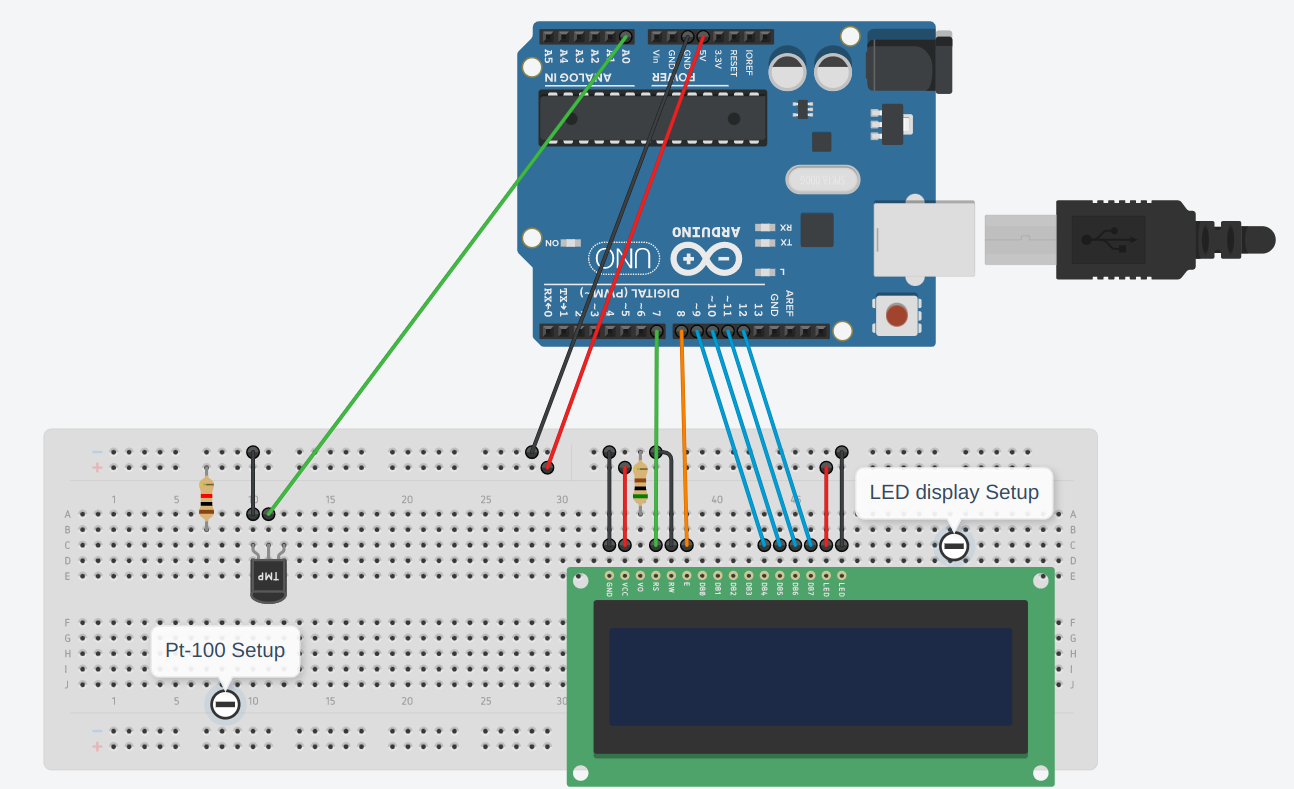
\includegraphics[scale = 0.22]{figs/Circuit.png}
    \caption{Circuit Diagram}
    \label{fig:2}
\end{figure}
\end{frame}

\begin{frame}{Training Data}
\begin{itemize}
\item The training data - Voltage reading of PT-100 collected from arduino and the Temperature reading collected from thermometer,  is shown in the following table \ref{tab:1}.

\begin{table}[h]
    \centering
    %%%%%%%%%%%%%%%%%%%%%%%%%%%%%%%%%%%%%%%%%%%%%%%%%%%%%%%%%%%%%%%%%%%%%%
%%                                                                  %%
%%  This is a LaTeX2e table fragment exported from Gnumeric.        %%
%%                                                                  %%
%%%%%%%%%%%%%%%%%%%%%%%%%%%%%%%%%%%%%%%%%%%%%%%%%%%%%%%%%%%%%%%%%%%%%%

\begin{center}
\begin{tabular}{|c|c|}
\hline
\textbf{Temperature (in $^{\circ}$C)} & \textbf{Voltage (in Volts)} \\ \hline
19      &   1.88 \\ \hline
25	    &   1.91 \\ \hline
36 		&   1.94 \\ \hline
42	    &   1.96 \\ \hline
50		&   2.00	 \\ \hline
79	    &   2.12 \\ \hline
84      &   2.14 \\ \hline
\end{tabular}
\end{center}

    \caption{Training Data}
  	\label{tab:1}
\end{table}
\end{itemize}
\end{frame}

%------------------------------------------------------------

\section{Optimization}
\begin{frame}{Least Squares Minimization}
	\begin{itemize}
	\item For $n$ data points $(x_1, y_1), (x_2, y_2), \ldots,(x_n, y_n)$, the least squares function is the sum of squares of the difference between observed and predicted data values, \\ 
	\begin{align}
		e &= \norm{\vec{y} - \vec{\hat{y}}}^2
	\end{align}
	where
	\begin{align}
		\vec{y} = \myvec{y_1 \\ y_2 \\ \vdots\\ y_n} \quad 
	\vec{\hat{y}} = \myvec{\hat{y}_{1} \\ \hat{y}_{2} \\ \vdots\\ \hat{y}_{n}}
	\end{align}
	$\hat{y_i}$ denotes the predicted value,
    ${y_i}$ denotes the observed value
	\end{itemize}
\end{frame}


\begin{frame}{Linear Modelling}
\begin{itemize}
\item The linear model is given by,
\begin{align}
	\hat{T}_{i} = w V_i + b
\end{align}
	\item For $n$ data points, we have
	\begin{align}
	\vec{\hat{T}} = \vec{V}^{\top}\vec{w}
	\end{align}
	where
	\begin{align}
		\vec{T} = \myvec{T_1 \\ T_2 \\ \vdots\\ T_n} \quad 
	\vec{\hat{T}} = \myvec{\hat{T}_{1} \\ \hat{T}_{2} \\ \vdots\\ \hat{T}_{n}} \quad
	\vec{V} = \myvec{V_1  & V_2 &  \ldots & V_n \\ 1 & 1 & \ldots &1}
	\quad
	\vec{w} = \myvec{w \\ b}
	\end{align}
\end{itemize}

\end{frame}

\begin{frame}{Optimization Problem Formulation}
\begin{itemize}

\item The optimization problem is given by
	\begin{align}
		\vec{w}_\text{opt} =  \arg\min_{\vec{w} \in \mathbb{R}^2}  \norm{\vec{T} - \vec{V}^{\top}\vec{w}}^2
	\end{align}
\item This optimization probelem can be solved using numpy.linalg.lstq, gradient descent, cvxpy. The codes for the same is given. All .algorithms give the same result
\end{itemize}
\end{frame}
%------------------------------------------------------------

\section{Results and Testing}
\begin{frame}{Linear Model Plot}
\begin{itemize}
\item The plot of the training data, linear model curve is shown in the figure \ref{fig:2}.
\begin{figure}[h]
    \centering
    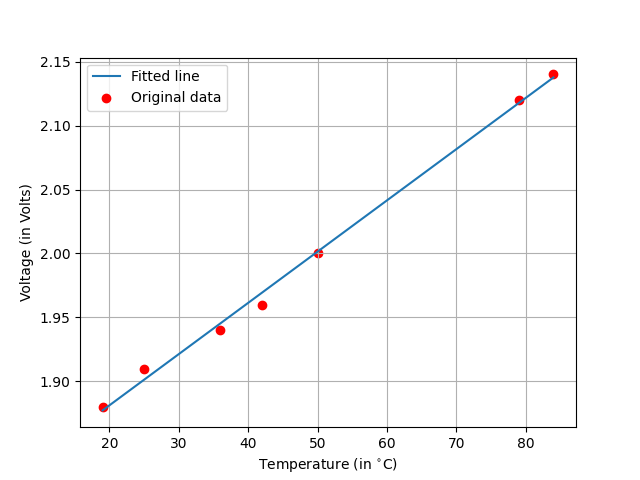
\includegraphics[scale = 0.48]{figs/Train.png}
    \caption{Model Training}
    \label{fig:2}
\end{figure}
\end{itemize}
\end{frame}


\begin{frame}{Results}
    \begin{itemize}
    \item The value of $\vec{w}_\text{opt}$ obtained from optimization is,
    \begin{align}
    \vec{w}_\text{opt} = \myvec{270.28248588 \\ -428.99096045}
    \end{align}
    
    \item Finally this $\vec{w}_\text{opt}$ is fed to the arduino so that the temperature displays on the LCD screen
    \end{itemize}
\end{frame}

\begin{frame}{Testing}
\begin{itemize}
    \item The data used to evaluate the model is shown in the following table \ref{tab:2}.

\begin{table}[h]
    \centering
    %%%%%%%%%%%%%%%%%%%%%%%%%%%%%%%%%%%%%%%%%%%%%%%%%%%%%%%%%%%%%%%%%%%%%%
%%                                                                  %%
%%  This is a LaTeX2e table fragment exported from Gnumeric.        %%
%%                                                                  %%
%%%%%%%%%%%%%%%%%%%%%%%%%%%%%%%%%%%%%%%%%%%%%%%%%%%%%%%%%%%%%%%%%%%%%%

\begin{center}
\begin{tabular}{|c|c|}
\hline
\textbf{Voltage (in Volts)} & \textbf{Temperature (in $^{\circ}$C)} \\ \hline
1.68 & 25 \\ \hline
1.72 & 35\\ \hline
1.77 & 50 \\ \hline
\end{tabular}
\end{center}

    \caption{Test Data}
    \label{tab:2}
\end{table}
\end{itemize}
\end{frame}

\begin{frame}{Linear Model Testing Plot}
\begin{itemize}
\item The test data, linear model curve are shown in the figure \ref{fig:3}.

\begin{figure}[ht]
    \centering
    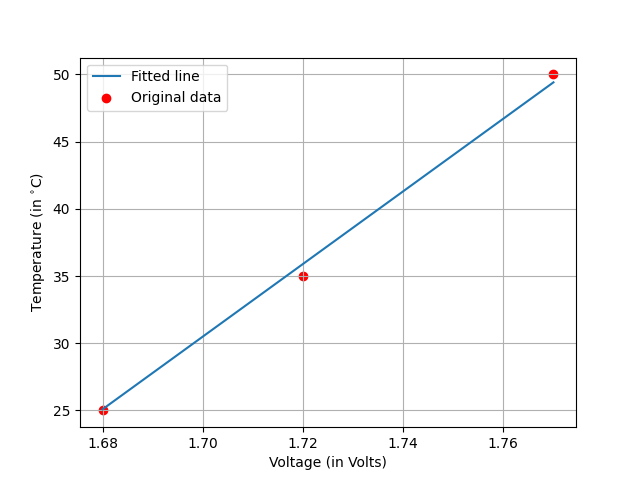
\includegraphics[scale = 0.48]{figs/Test.png}
    \caption{Model Evaluation}
    \label{fig:3}
\end{figure}
\end{itemize}
\end{frame}

\section{Conclusion}
\begin{frame}{Conclusion}
\begin{itemize}
\item In conclusion, this project effectively used machine learning to model the voltage-temperature characteristics of the PT-100, utilizing the least squares method and validating the model through test data. \vspace{0.25cm}
\item The project showcases the practical implementation of data collection and optimization.
\end{itemize}
\end{frame}

\end{document}